\documentclass[twoside,11pt]{article}
\usepackage{jmlr2e}
\usepackage{graphicx}
\graphicspath{ {./images/} }
\usepackage{enumitem}
\newlist{mylistenv}{enumerate}{3}
\newenvironment{mylist}[1]{%
	\setlist[mylistenv]{label=#1\arabic{mylistenvi}.,ref=#1\arabic{mylistenvi}}%
	\setlist[mylistenv,2]{label=#1\arabic{mylistenvi}.\arabic{mylistenvii}.,ref=#1\arabic{mylistenvi}.\arabic{mylistenvii}}%
	\setlist[mylistenv,3]{label=#1\arabic{mylistenvi}.\arabic{mylistenvii}.\arabic{mylistenviii}.,ref=#1\arabic{mylistenvi}.\arabic{mylistenvii}.\arabic{mylistenviii}}%
	\renewenvironment{mylist}{\begin{mylistenv}}{\end{mylistenv}}
	\begin{mylistenv}%
	}{%
	\end{mylistenv}%
}
\newcommand\tab[1][1cm]{\hspace*{#1}}

% Definitions of handy macros can go here

\newcommand{\dataset}{{\cal D}}
\newcommand{\fracpartial}[2]{\frac{\partial #1}{\partial  #2}}


\firstpageno{1}

\begin{document}

\title{Project 5: Reinforcement Learning}

\author{\name Sarah Wilson 
	   \email swi1s117@jhu.edu \\
	   \phone 303-921-7225 \\
       \addr Engineering Professionals Computer Science\\
       Johns Hopkins University\\
       Baltimore, MD 21218, USA} 

%S\maketitle


\section{Introduction}
\hspace*{10mm} Reinforcement Learning (RL) is an area of Machine Learning that uses experiences to determine the next optimal decision. Typical the reinforcement learning process can be broken down into a few key steps: Observe the environment, decide how to act based on a policy, act based on that policy, be rewarded or penalized for that action, update the policy, iterate until the best policy is produced. Two major type of RL algorithms are the model-based and model-free algorithms. In the model-based algorithms a the function used to issue the reward is used to determine the best policy. \\


\hspace*{10mm} The objective of this paper is to explore three different reinforcement learning algorithms, Value Iteration, Quality Learning or Q-Learning and the State Action Reward State Action (SARSA) algorithm. These algorithms will be explored and implemented through the racetrack problem. In the racetrack problem, the objective is to get a car from the starting line to the finish line in as little time as possible. The racetrack will be described as a two dimensional Cartesian plane, where the location of the car on the racetrack can be described as a point pair $(x,y)$. The active control exerted over the car will be acceleration $a_x$ and $a_y$. The range of values that can be assigned to $a_x$ and $a_y$ are -1,0,1. The velocity of the car will be capped to values between -5 and 5, any acceleration values that cause the velocity to go beyond these bounds will be ignored. Additional the probability of the acceleration control being applied on each time step is 80\%, meaning there is a 20\% chance the accelerate control is issued no acceleration updates will occur. The experiments for these algorithms will occur on three uniquely shaped racetracks, the R-Shaped, O-Shaped and L-Shaped tracks.\\ 

\hspace*{10mm} An additional constraint that will be applied to this problem, is the consequence of a crash. A crash is defined as the car intersecting with the walls of the racetrack, in one variation if a crash happens, the car will be placed back to a location on the track nearest to the crash site with a zero velocity component. In the second, harsher variation, if a crash happens, the car will be placed back at the start of the racetrack with a zero velocity component. These variations will only be applied to the R-Shaped race track, the O-Shaped and L-Shaped tracks will not implement the harsher variation of the crash, instead if a crash occurs on these tracks the car will be placed at a location nearest to the crash site. \\

\hspace*{10mm} The hypothesis presented in this paper predicts that the SARSA algorithm will perform better compared to the Q-Learning or Value Iteration algorithms. The reason for this hypothesis is that the SARSA algorithm is an on-policy algorithm as it updates the policy based on the current choices of the policy that is being implemented. The Q-Learning algorithm, however, does not update the same policy used to explore the world. The SARSA algorithm seems better suited for the racetrack problem, since the actions taken by the model to drive the car the fastest around the racetrack should update the policy as the world is better understood, if the model understand there is a wall or turn coming up, it will have the environment baked into the policy, where as the Q-Learning or Value Iteration algorithms, do not account for updates to the environment each time the policy is updated.\\ 

\hspace*{10mm} Section 1 has provided the introduction, problem statement and hypothesis in regards to three major learning algorithms that will be explored. Section 2 will provide an in-depth explanation of the algorithms. Section 4 will present the results obtained by the different algorithms. Section 5 will discuss the results that were obtained and compare them to the hypothesis that was outlined in the introduction. This report will conclude in Section 6 with a discussion of lessons learned and areas of possible future work.\\

\newpage

\section{Algorithms and Experimental Methods}
\textbf{Value Iteration}\\
\hspace*{10mm} Value Iteration is one type of Reinforcement Learning. In Value Iteration the Value $V(s)$ represents how good a state the agent is currently in, typically the higher the value the best position the agent is in. The value function is dependent on the policy that the agent used to get into a given state. For a given set of states (s) that belong to the set State Space (S) there is a maximum value where the value of that state is highest among all states in the State Space. This value has an optimal policy associated with it. The $Q$ Function is a representation of the total expected reward received by an agent in state s and picking an action (a) out of the whole Action Space (A). In Value Iteration the agent is not involved in the process of learning, instead the optimal state is determined by iterating and improve the estimate of $V(s)$ until the different between iterations on $V(s)$ is within a certain value, at this point the algorithm is considered converged and the car can be run using the policy obtained during the training. The general algorithmic steps for the Value Iteration Algorithm are shown below:\\
\textbf{Value Iteration}\\
Train the Car:\\
\tab For all states ($s$) in the overall State Space (S):\\
\tab \tab Set $V(s)$ to $0$\\
\tab While  $max_{s of S}(V_t(s) - V_{t-1}(s)) < \epsilon$:\\
\tab \tab Number of Iterations = Number of Iterations + 1\\
\tab \tab For all states ($s$) in the overall State Space (S):\\
\tab \tab \tab For all actions ($a$) in the overall Action Space (A):\\
\tab \tab \tab \tab $Expected Value = 0.8 * (V(Acc Applied)) + 0.2 * (V(Acc Not Applied))$\\
\tab \tab \tab \tab $Q_t(s,a) = Reward + \eta*(Expected Value) * V_{t-1}(s')$\\
\tab \tab \tab $\pi_t(s) = max_{a of A}(Q_t(s,a))$\\
\tab \tab \tab $V_t(s) = Q_t(s,\pi_t(s))$\\
\\
Test the Car:\\
\tab While the Car has not reached the finish line:\\
\tab \tab Get Best Policy (Acceleration) based on Current State\\
\tab \tab Apply Acceleration to Car and Update Velocity and Position\\
\tab \tab Check Car if the Car has hit a wall\\
\tab \tab If Wall Hit has Occurred:\\
\tab \tab \tab If the Crash is Type 1:\\
\tab \tab \tab \tab Place the Car back to the near position of the crash\\ 
\tab \tab \tab \tab and set velocity to zero.\\
\tab \tab \tab If the Crash is Type 2:\\
\tab \tab \tab \tab Place the Car back to at starting position and set velocity to zero.\\
\newpage

\textbf{Q-Learning}\\
INSERT GENERAL DESCRIPTION.\\
The general algorithmic steps for the Q-Learning Algorithm are shown below:\\

\textbf{Q-Learning}\\
Train the Car:\\
\tab Initialize all $Q(s,a)$ to -1000.\\
\tab Set a number of Training Iterations (Episodes)\\
\tab For each Training Iteration in the total number of Training Iterations:\\
\tab \tab Initialize s by setting the car to the starting position.\\
\tab \tab While the Car has not has not reached the finish line or the maximum number of moves has not been reached\\
\tab \tab \tab Chose an Action (a) from Q(s,a) based the current state using an $\epsilon$ Greedy Approach \\
\tab \tab \tab $\epsilon$ Greedy Approach:\\
\tab \tab \tab \tab Chose action a based on the best policy
\tab \tab \tab \tab Or\\
\tab \tab \tab \tab Randomly pick the action from the Action Space\\
\tab \tab \tab Take action (a) observe the reward and update the cars state.\\
\tab \tab \tab Update $Q(s,a)$:\\
\tab \tab \tab \tab  $Q(s,a) = Q(s,a) + \eta*(reward + \gamma*max_{a'}Q(s',a') - Q(s,a))$\\
\\
Test the Car:\\
\tab While the Car has not reached the finish line:\\
\tab \tab Get Best Policy (Acceleration) based on Current State\\
\tab \tab Apply Acceleration to Car and Update Velocity and Position\\
\tab \tab Check Car if the Car has hit a wall\\
\tab \tab If Wall Hit has Occurred:\\
\tab \tab \tab If the Crash is Type 1:\\
\tab \tab \tab \tab Place the Car back to the near position of the crash\\ 
\tab \tab \tab \tab and set velocity to zero.\\
\tab \tab \tab If the Crash is Type 2:\\
\tab \tab \tab \tab Place the Car back to at starting position and set velocity to zero.\\
\newpage

\textbf{SARSA}\\
State-Action-Reward-State-Action (SARSA) is the final type of Reinforcement Learning algorithm that will be discussed in this paper. SARSA is an on-policy learning algorithm, it is on-policy because it chooses the action for each state while the learning is occurring and does so by following the policy. This is the biggest different between Q-Learning and SARSA, SARSA learns and updates while following the policy, Q-Learning does not. Stated differently \\

\textbf{SARSA}\\
Train the Car:\\
\tab Initialize all $Q(s,a)$ to -1000.\\
\tab Unless state position is a finish spot, then sent $Q(finish,a)$ to zero.\\
\tab Set a number of Training Iterations (Episodes)\\
\tab For each Training Iteration in the total number of Training Iterations:\\
\tab \tab Initialize s by setting the car to the starting position.\\
\tab \tab Chose an Action (a) from Q(s,a) based the current state using an $\epsilon$ Greedy Approach \\
\tab \tab While the Car has not has not reached the finish line or the maximum number of moves has not been reached\\
\tab \tab \tab Take action (a) observe the reward and update the cars state to s'.\\
\tab \tab \tab Chose a second action (a') from state s' using using an $\epsilon$ Greedy Approach\\
\tab \tab \tab $Q(s,a) = Q(s,a) + \eta*(reward + \gamma * Q(s',a') - Q(s,a))$\\
\\
Test the Car:\\
\tab While the Car has not reached the finish line:\\
\tab \tab Get Best Policy (Acceleration) based on Current State\\
\tab \tab Apply Acceleration to Car and Update Velocity and Position\\
\tab \tab Check Car if the Car has hit a wall\\
\tab \tab If Wall Hit has Occurred:\\
\tab \tab \tab If the Crash is Type 1:\\
\tab \tab \tab \tab Place the Car back to the near position of the crash\\ 
\tab \tab \tab \tab and set velocity to zero.\\
\tab \tab \tab If the Crash is Type 2:\\
\tab \tab \tab \tab Place the Car back to at starting position and set velocity to zero.\\
\newpage


\section{Data Sets}
\hspace*{10mm} For this paper there were no explicate data-sets provided. Instead the data provided was in the form of the shape of the Racetracks. There were three uniquely shaped racetracks, the R-Shaped, O-Shaped and L-Shaped tracks provided for this problem. Each taking on the shape of the letter in their respective names.\\
	
\section{Results}
\hspace*{10mm} Tables 1-3 display the learning for each of the algorithms across both types of crash variations. For brevity of this report the processing of tuning the various tune parameters (Learning Rate, Discount Factor, ect) have been omitted.\\ 
Table 1 shows the Learning Curve for Value Iteration, the optimal values used to obtain these results were: $\epsilon = 0.000001$, Discount = 0.7, Limit On Iterations = 1000. Note the Limit on Iterations was set just in case the algorithm values different did not converge in a reasonable amount of time, in all runs obtained for this report the Limit of Iterations was never hit.\\
Table 2 shows the Learning Curve for Q-Learning, the optima values used to obtain these results were: $\epsilon = 0.02$, Discount = 0.9, Learning Rate = 0.6, Maximum Number of Moves = 1000, Number of Training Runs = 10,000. The Maximum Number of Moves was put in place to limit how long the car was allowed to explore the environment during each training run.\\
Table 3 shows the Learning Curve for SARSA, the optima values used to obtain these results were: $\epsilon = 0.02$, Discount = 0.9, Learning Rate = 0.6, Maximum Number of Moves = 1000, Number of Training Runs = 10,000. The Maximum Number of Moves was put in place to limit how long the car was allowed to explore the environment during each training run.\\
Table 4 shows the results of the Test Runs for each of the algorithms and the crash variations, to get a statstical analysis the car was run using the policy obtained during training 10 times. The number of moves required to complete the track was then averaged to provide the numbers in Table 4. Note that Q-Learning and SARSA both had a hard cap of 1,000 moves that they were allowed to utilized while the test ran.\\  

\begin{table}[h]
	\centering
	\caption{Value Iteration, Q-Learning and SARSA Average Moves Taken Across 10 Cars}
	\label{tab:table4}
	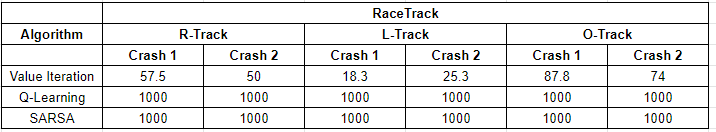
\includegraphics[scale=.8]{RunTimeComp_All}\newline
\end{table}

\newpage

\begin{table}[h]
		\centering
		\caption{Value Iteration Learning Curves All Race Tracks }
		\label{tab:table1}
		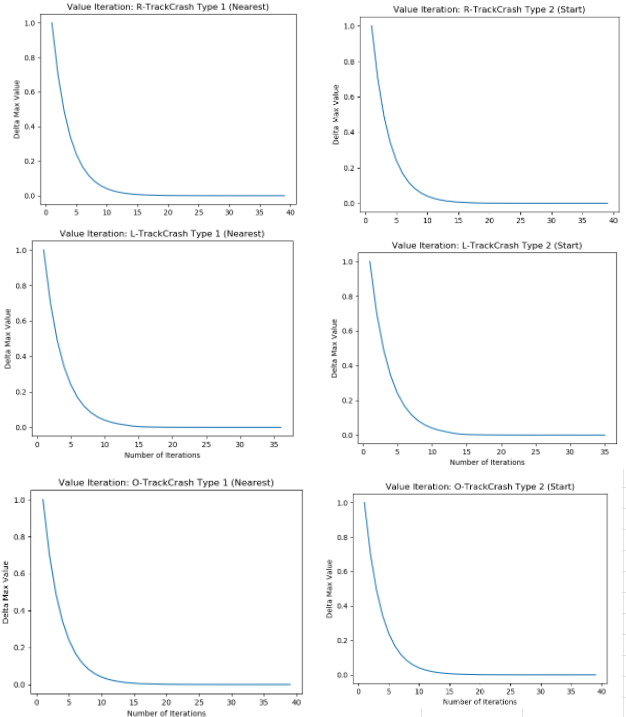
\includegraphics[scale=1]{ValIter_All_TrainCurve}\newline
\end{table}

\newpage

\begin{table}[h]
	\centering
	\caption{Q Learning Learning Curves All Race Tracks }
	\label{tab:table2}
	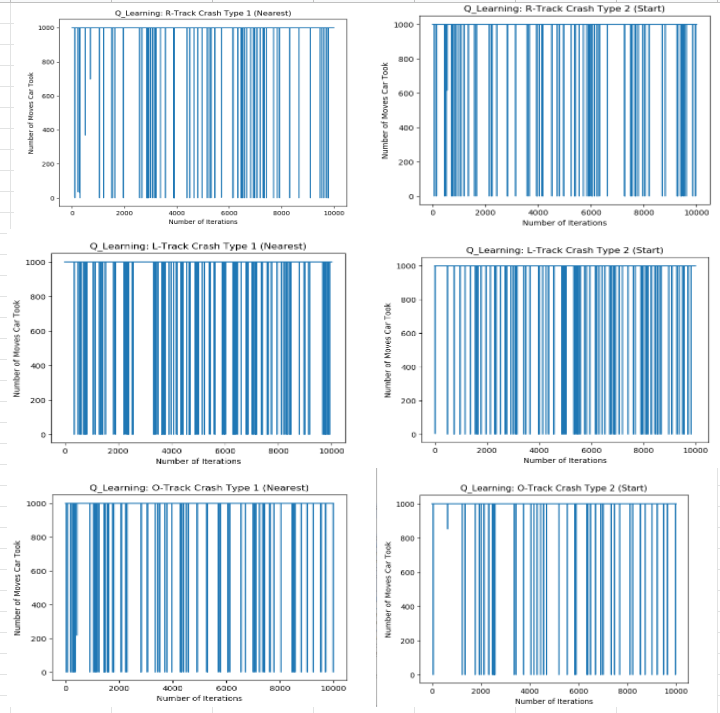
\includegraphics[scale=.9]{Q_All_TrainCurve}\newline
\end{table}

\newpage

\begin{table}[h]
	\centering
	\caption{SARSA Learning Learning Curves All Race Tracks }
	\label{tab:table3}
	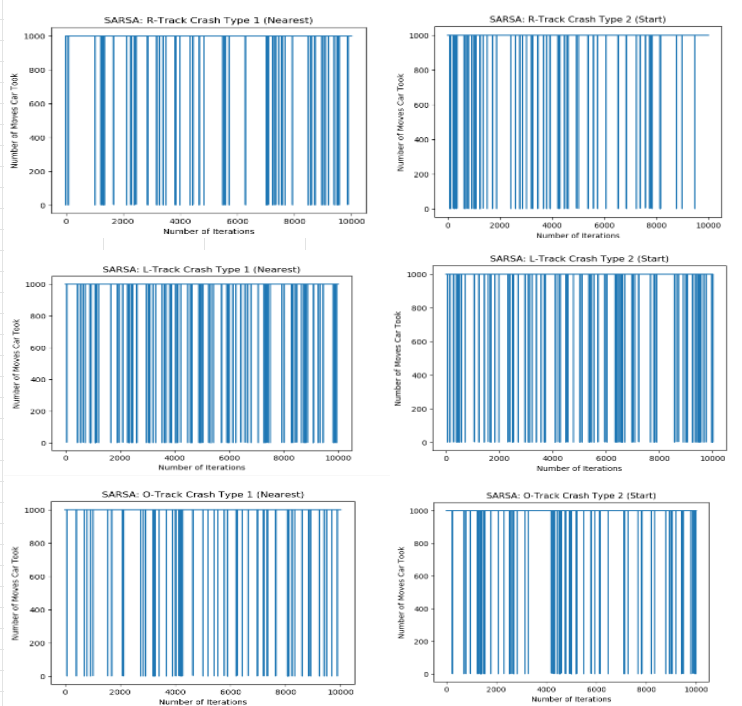
\includegraphics[scale=.9]{SARSA_All_TrainCurve}\newline
\end{table}

\newpage

\section{Discussion}
\hspace*{10mm} The hypothesis presented in this report was that the SARSA algorithm will perform better compared to the Q-Learning or Value Iteration algorithms.\\

\section{Conclusion}
\hspace*{10mm} Overall, the results could not provide meaningful data towards the hypothesis that SARSA would out perform Q-Learning or Value Iteration. The only comparisons that can be drawing is by examining the data obtained for the learning curves during the training runs. In general, the difference between the two crash variations did cause the cars to learn different behavior. In Q-Learning and SARSA, when the car was placed back at a nearest location to the crash, the car was more often able to finish the racetrack during the training iterations. During the course of these experiments it was noticed that the seed values for Epsilon, Q and Learning Rate also produced drastically different results. A lesson learned from this project is to have a fun understanding of what part of the algorithm these parameters impact prior to running the algorithm, as a bad seed value can lead to lost time in trying to debug an implementation issue that simply isn't there, instead poorly chosen values are making it appear as if the algorithm is not running correctly.\newline
\hspace*{10mm} A suggested area of future work, aside from fixing the implementation issues that might have been altering the results obtained for the Q-Learning and SARSA algorithms, would be to explore the impact of varying the starting position of the car on each training iteration of the Q-Learning and SARSA algorithms. If the initialized position of the car was varied on each iteration or the initialized position was placed closure to the finish line and then worked back towards the start lining, it is possible that the Values of Q would have percolated backwards towards the start, providing the car with the motivation (value insecntive) to move towards the finish line. This could also be the root cause of the implementation issue that was impacting the Q-Learning and SARSA algorithms. \newline

\section{References}
1. Alpaydin, E. (2004). Introduction to machine learning (Oip). Mit Press. 

\newpage


\end{document}